\section{Frontend Functionality} \label{sec:frontend-functionality}
The frontend makes the SAT solver accessible through an interactive interface.
The user can configure the problem without manually writing SAT clauses or JSON requests.

\subsection{Problem Setup Panel} \label{subsec:problem-setup-panel}

The problem setup panel allows the user to select:

\begin{itemize}
    \item the task type,
    \item the total number of floors,
    \item the number of movers,
    \item item names and initial item floors,
    \item custom mover names,
    \item target floors for Task 1,
    \item solving mode,
    \item maximum number of steps or exact time horizon.
\end{itemize}

\noindent For Task 1, advanced options allow the user to set target floors for each mover.
For Task 2, the target is fixed: every mover and every item must finish on floor $0$.

\subsection{Results Panel} \label{subsec:results-panel}

After the solver runs, the results panel displays whether the instance is satisfiable or unsatisfiable.
If a solution exists, the panel shows:

\begin{itemize}
    \item the solve ID,
    \item the solver runtime,
    \item the optimal number of steps,
    \item buttons for downloading the DIMACS CNF and mapping,
    \item playback controls for the solution timeline.
\end{itemize}

\subsection{Building Visualizer} \label{subsec:building-visualizer}

The building visualizer represents the floors graphically.
Movers are shown as person icons, while items are shown as boxes.
At each time step, the visualizer updates the positions of all persons and items according to the decoded SAT model.

\begin{figure}[H]
    \centering
    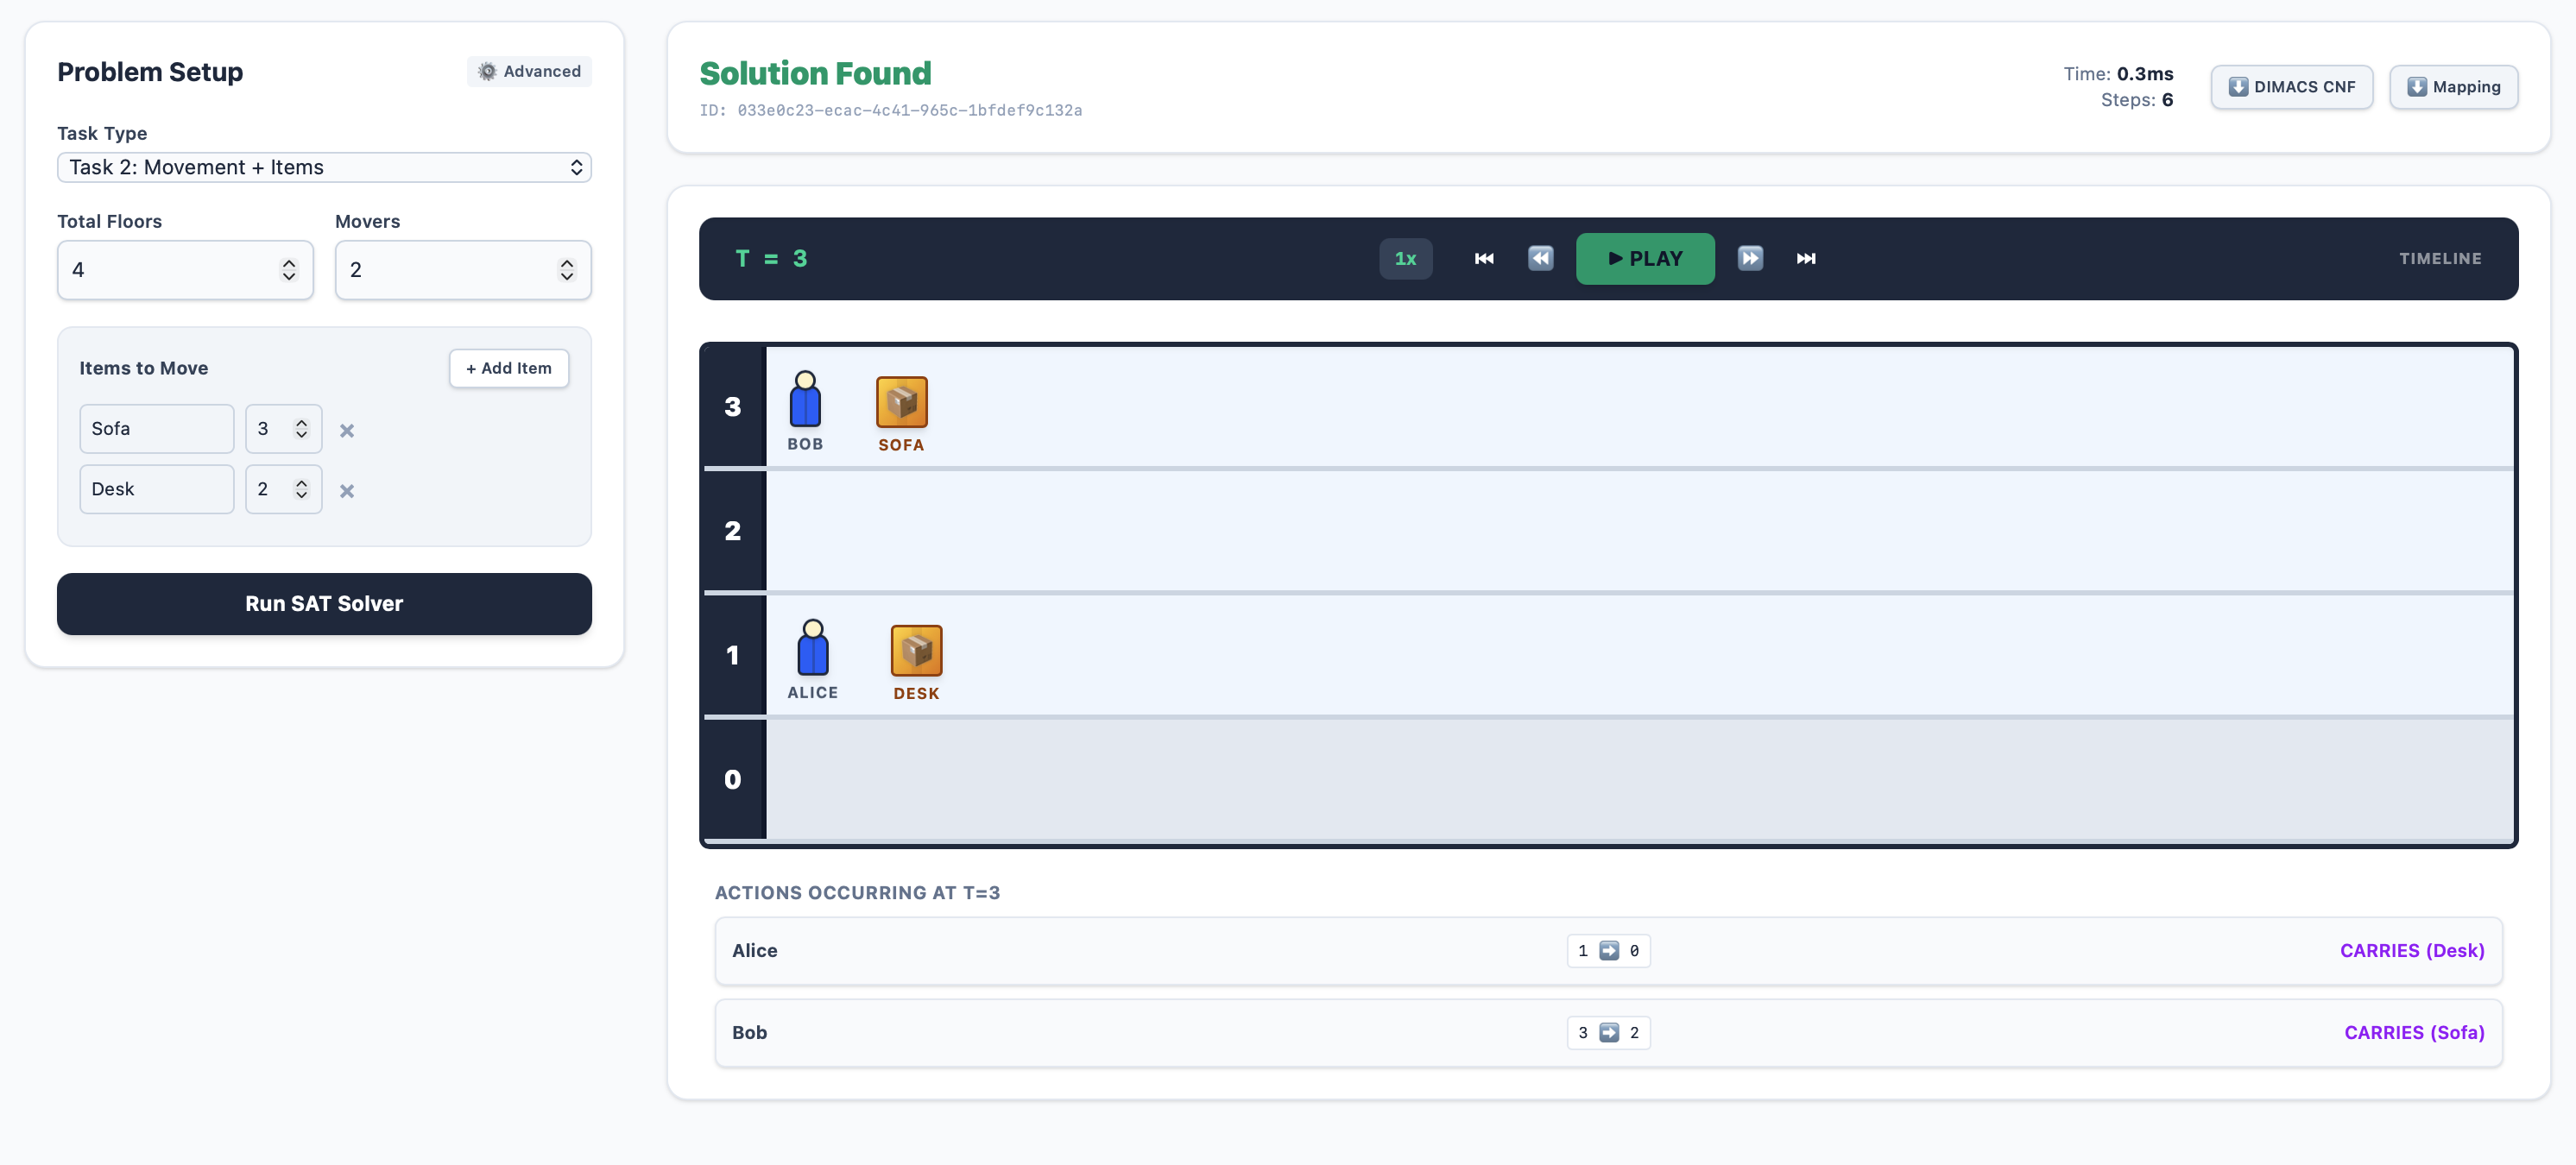
\includegraphics[width=0.95\textwidth]{figures/task2-frontend-overview}
    \caption{Frontend visualization of a satisfiable Task 2 instance with two movers and two items.}
    \label{fig:frontend-sat}
\end{figure}

\subsection{Action Log}

The action log describes what happens at the selected time step.
For example, it may show that Alice descends from floor $2$ to floor $1$, or that Bob carries a table from floor $1$ to floor $0$.